% Section 1 - Introduction
% Roberto Masocco <roberto.masocco@uniroma2.it>
% May 6, 2024

% ### Introduction ###
\section{Introduction}
\graphicspath{{figs/section1/}}

% --- Information ---
\begin{frame}{Information}
	\begin{itemize}
		\item \textbg{Calendar}: from May 9 to June 13, 2024, see Teams for schedule.
		\item \textbg{Topics}:
		      \begin{enumerate}
			      \item Middleware for robotics and more.
			      \item Development tools for robotics (\emph{e.g.}, Docker).
			      \item The MARTe2 framework for real-time control architectures in tokamaks.
		      \end{enumerate}
		\item \textbg{Materials}:
		      \begin{itemize}
			      \item Code repository: \href{https://github.com/IntelligentSystemsLabUTV/ros2-examples}{\color{blue}\underline{github.com/ros2-examples}} (\texttt{humble} branch).
			      \item Lectures: \href{https://github.com/stars/robmasocco/lists/lectures}{\color{blue}\underline{github.com/robmasocco}}, Teams directory (this lecture is \href{https://github.com/robmasocco/DAFN24_Robotics_1}{\color{blue}\underline{here}}).
		      \end{itemize}
		\item \textbg{Useful background}:
		      \begin{itemize}
			      \item Basics of C and Python programming.
			      \item Basics of Git workflow (check out \href{https://www.atlassian.com/git/tutorials/what-is-git}{\color{blue}\underline{this tutorial}} by Atlassian).
			      \item Everyday Linux commands and a Unix-like system.
		      \end{itemize}
		      \visible<2>{
		\item \textbg{Exam}: ... ask Prof. Carnevale \smiley~some projects will be proposed later on.
		      }
	\end{itemize}
\end{frame}

% --- Program ---
\begin{frame}{Program}
	\begin{enumerate}
		\item Roboticist 101 - Software and middleware for robotics
		\item ROS 2 - Workflow and basic communication
		\item ROS 2 - Advanced communication
		\item ROS 2 - Node configuration
		\item ROS 2 - Sensor sampling and image processing
		\item Localization and mapping - From EKF to SLAM
		\item Inside the roboticist's toolbox - Linux kernel, Docker, and more
		\item microROS - Bridging the gap
		\item MARTe2 - A real-time control framework for nuclear fusion
	\end{enumerate}
\end{frame}

% --- Survey ---
\begin{frame}{Survey}
  Please answer without fear!\\
  \bigskip
  Who knows what about:
  \begin{itemize}
    \visible<2->{\item Version control and Git?}
    \visible<3->{\item Python?}
    \visible<4->{\item C/C++, from coding to linking?}
    \visible<5->{\item Object-oriented programming?}
    \visible<6->{\item Networking and the ISO/OSI model?}
    \visible<7->{\item Extended Kalman Filter and variants?}
  \end{itemize}
\end{frame}

% --- The roboticist ---
\begin{frame}{The roboticist}{A new path for control engineers}
	\begin{columns}
		\column{.5\textwidth}
		A \textbg{control engineer} is a specialist in the \textbg{design} of controllers to drive \textbg{dynamic systems}; the implementation was traditionally left to other specialists.\\
		A \textbg{roboticist} is a specialist capable of designing, \textbg{building}, and \textbg{programming} complex \textbg{autonomous systems}; with skills ranging from computer science to other disciplines.
		\begin{block}{}
			\centering
			\textbf{A control engineer can be very effective as a roboticist.}
		\end{block}

		\column{.5\textwidth}
		\begin{figure}
			\centering
			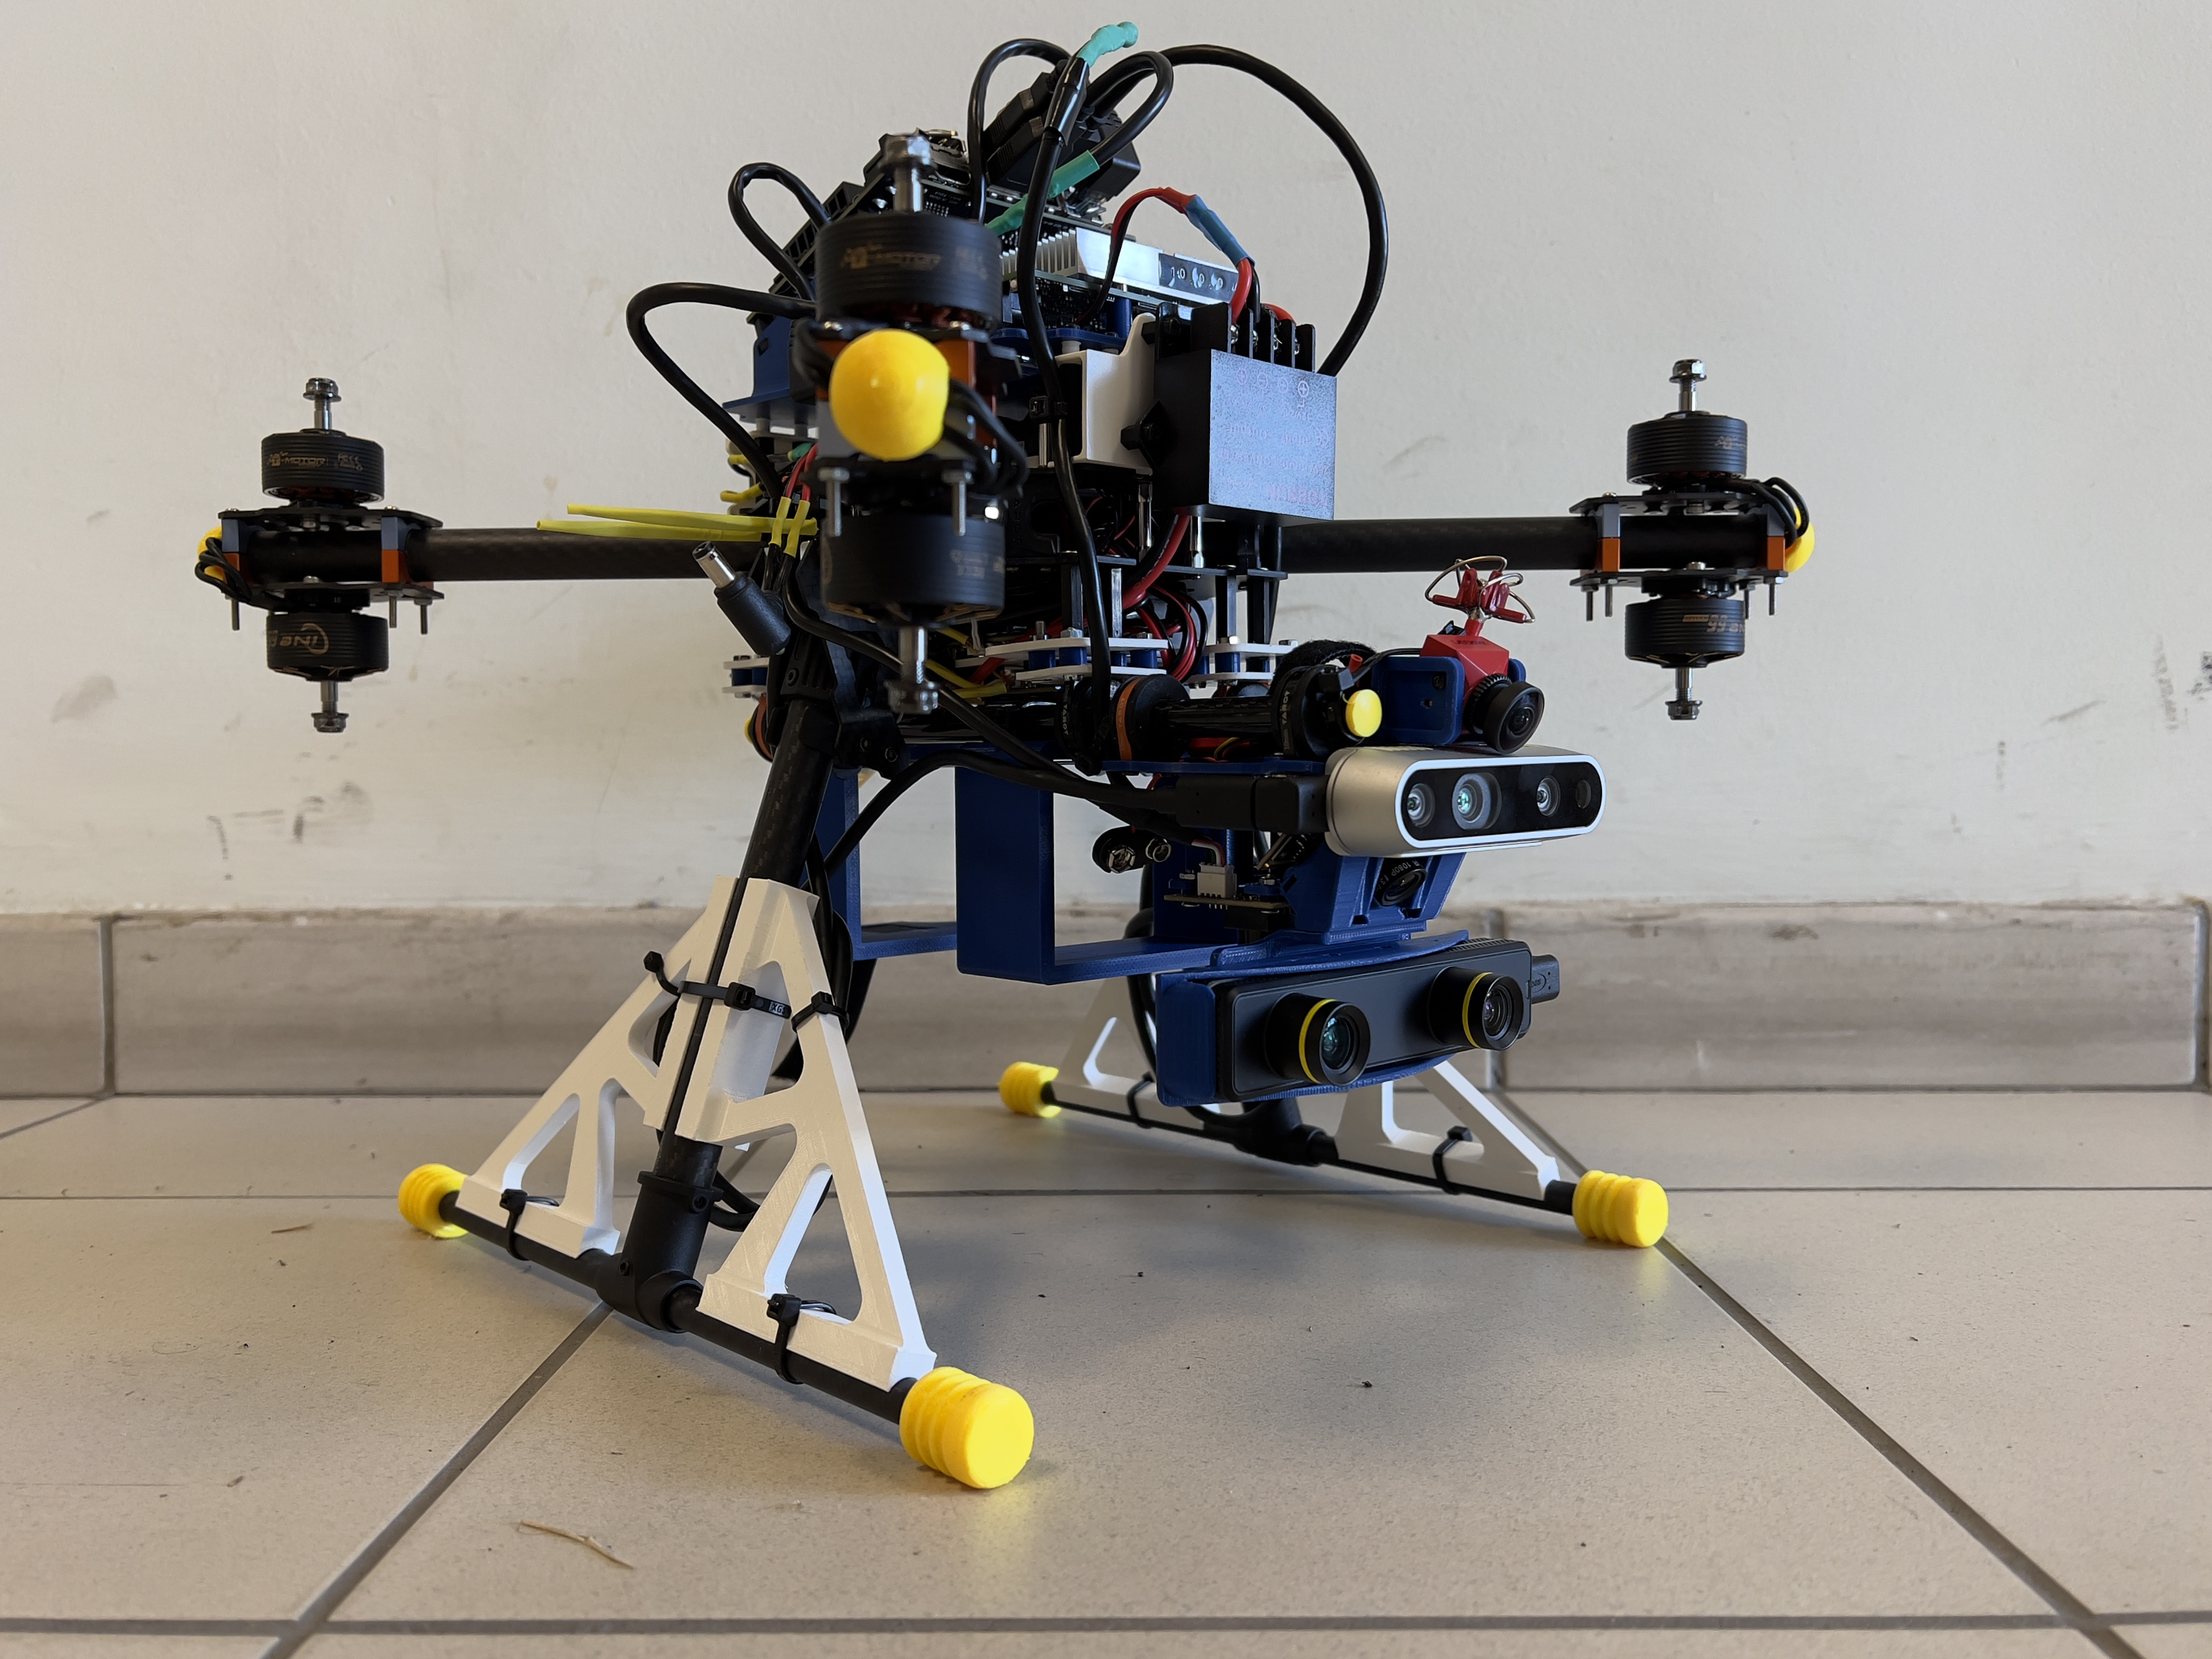
\includegraphics[width=.8\textwidth]{stanis}
			\caption{Stanis autonomous drone prototype.}
			\label{fig:stanis}
		\end{figure}
	\end{columns}
\end{frame}
\begin{frame}{The roboticist}{A new path for control engineers}
	\begin{columns}
		\column{.5\textwidth}
		A \textbg{roboticist} can usually:
		\begin{itemize}
			\item \textbg{design} solutions to complex problems;
			\item \textbg{develop} parts of a robot, or entire \textbg{control architectures};
			\item \textbg{deploy} and test software and hardware solutions;
			\item make use of modern \textbg{hardware accelerators} and robotics-oriented hardware.
		\end{itemize}
		Industries are looking for roboticist for their \textbg{versatile skill set}.

		\column{.5\textwidth}
		\begin{figure}
			\centering
			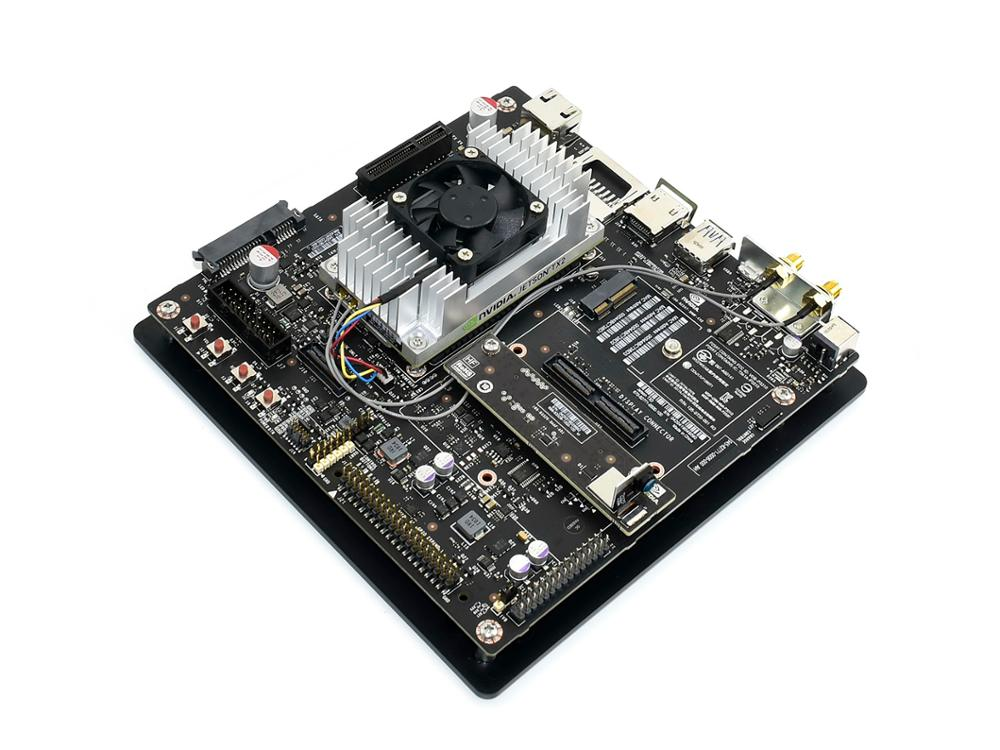
\includegraphics[width=.9\textwidth]{tx2}
			\caption{Nvidia Jetson TX2 developer kit.}
			\label{fig:tx2}
		\end{figure}
	\end{columns}
\end{frame}
